% Editable standalone vector figure extracted from spectra.tex.
% Source slide 24; figure 23; native embedded fonts.
% Compile with LuaLaTeX from this directory, or run ../export_figures.py.
\documentclass[tikz,border=0pt]{standalone}
% Shared editable preamble for standalone, Nature-style vector figures.
% Text remains embedded and searchable. This is a house-style target, not a
% claim of acceptance or of satisfying every journal's submission checklist.
\usepackage{fontspec}
\setmainfont{LiberationSans}[
  Path=../../shared/assets/,Extension=.ttf,
  UprightFont=*-Regular,BoldFont=*-Bold,ItalicFont=*-Italic,BoldItalicFont=*-BoldItalic]
\setsansfont{LiberationSans}[
  Path=../../shared/assets/,Extension=.ttf,
  UprightFont=*-Regular,BoldFont=*-Bold,ItalicFont=*-Italic,BoldItalicFont=*-BoldItalic]
\setmonofont{LiberationSans}[
  Path=../../shared/assets/,Extension=.ttf,
  UprightFont=*-Regular,BoldFont=*-Bold,ItalicFont=*-Italic,BoldItalicFont=*-BoldItalic]
\usepackage{unicode-math}
\setmathfont{Latin Modern Math}
\DeclareMathSizes{5.9}{6}{5}{5}
\DeclareMathSizes{6}{6}{5}{5}
\usepackage{tikz}
\usetikzlibrary{arrows.meta,calc,positioning,patterns,decorations.pathreplacing,matrix}
\usepackage{graphicx}
\usepackage{xcolor}
\pagecolor{white}
\definecolor{ink}{HTML}{202020}
\definecolor{paper}{HTML}{FFFFFF}
\definecolor{muted}{HTML}{494949}
\definecolor{line}{HTML}{808080}
\definecolor{soft}{HTML}{F0F0F0}
\hyphenpenalty=10000\exhyphenpenalty=10000
\newcommand{\figurefont}{\sffamily\fontsize{5.9}{7.4}\selectfont}
\newcommand{\figuremathfont}{\sffamily\fontsize{6}{7.5}\selectfont}
\newcommand{\brandmedium}{\bfseries}
\renewcommand{\normalsize}{\figurefont}
\renewcommand{\small}{\figurefont}
\renewcommand{\footnotesize}{\figurefont}
\renewcommand{\scriptsize}{\figurefont}
\renewcommand{\tiny}{\figurefont}
\renewcommand{\large}{\figurefont}
\renewcommand{\Large}{\figurefont}
\renewcommand{\LARGE}{\figurefont}
\renewcommand{\huge}{\figurefont}
\renewcommand{\Huge}{\figurefont}
\tikzset{
  every path/.style={line width=.55pt},
  every node/.style={font=\figurefont,text=ink},
  arr/.style={-{Latex[length=1.5mm,width=1mm]},line width=.55pt,draw=ink},
  thinarr/.style={-{Latex[length=1.3mm,width=.9mm]},line width=.55pt,draw=ink},
  box/.style={draw=ink,line width=.55pt,fill=white,minimum height=.85cm,align=center,inner sep=3pt},
  ghost/.style={draw=muted,dashed,fill=soft},
  tag/.style={font=\figurefont,text=muted},
  equ/.style={font=\figuremathfont},
  small/.style={font=\figurefont},
  body/.style={font=\figurefont},
  tinytext/.style={font=\figurefont}
}
\newcommand{\txt}[4]{\node[anchor=north west,align=left,text width=#3cm] at (#1,#2) {#4};}
\newcommand{\smalltxt}[4]{\node[anchor=north west,align=left,text width=#3cm,small] at (#1,#2) {#4};}
\newcommand{\eqn}[4][6]{\node[anchor=north west,font=\figuremathfont] at (#2,#3) {$\displaystyle #4$};}
\newcommand{\diagramblock}[5]{\node[box,minimum width=#3cm,text width=#3cm,minimum height=#4cm] at (#1,#2) {#5};}
% Scale coordinates, not text: all labels retain one final publication size.
\newcommand{\spectrum}[3]{\begin{scope}[shift={(#1,#2)}]
  \draw[muted] (0,0)--({3.6*#3},0);
  \draw[muted] (0,0)--(0,{1.9*#3});
  \foreach \x/\h in {.25/.18,.49/.46,.68/1.42,.87/.37,1.08/.74,1.31/.31,1.57/1.78,1.76/.46,1.96/.19,2.17/1.1,2.37/.57,2.57/.31,2.88/.76,3.21/.23,3.4/.38}{
    \draw[ink] ({\x*#3},0)--({\x*#3},{\h*#3});}
  \foreach \x in {.6,1.2,1.8,2.4,3.0}{\draw[ink] ({\x*#3},0)--+(0,{-.06*#3});}
  \foreach \y in {.45,.9,1.35,1.8}{\draw[ink] (0,{\y*#3})--+({-.06*#3},0);}
  \foreach \x/\lab in {0/0,1.8/45,3.6/90}{\node[anchor=north,font=\figurefont] at ({\x*#3},{-.08*#3}) {\lab};}
  \foreach \y/\lab in {0/0,.9/0.5,1.8/1.0}{\node[anchor=east,font=\figurefont] at ({-.08*#3},{\y*#3}) {\lab};}
  \node[anchor=north east,font=\figurefont] at ({3.6*#3},{-.45*#3}) {$m/z$ (Th)};
  \node[anchor=south west,font=\figurefont] at (0,{1.96*#3}) {Relative intensity (a.u.)};
\end{scope}}
\newcommand{\molecule}[3]{\begin{scope}[shift={(#1,#2)}]
  \draw[ink] (0,{#3})--({.866*#3},{.5*#3})--({.866*#3},{-.5*#3})--(0,{-#3})--({-.866*#3},{-.5*#3})--({-.866*#3},{.5*#3})--cycle;
  \draw[ink] ({.68*#3},{.4*#3})--({.68*#3},{-.4*#3});
  \draw[ink] ({-.7*#3},{-.44*#3})--({-.02*#3},{-.83*#3});
  \draw[ink] ({-.7*#3},{.44*#3})--({-.02*#3},{.83*#3});
  \draw[ink] (0,{#3})--(0,{1.55*#3});
  \node[font=\figurefont] at (0,{1.77*#3}) {OH};
\end{scope}}
\newcommand{\peaktokens}[3]{\foreach \i in {0,...,5}{\pgfmathsetmacro{\xx}{#1+\i*.36}\draw[fill=#3,draw=ink] (\xx,#2) rectangle +(.24,.6);}}
\newcommand{\E}{\mathbb E}
\newcommand{\R}{\mathbb R}
\newcommand{\sg}{\operatorname{stopgrad}}
\newcommand{\LN}{\operatorname{LN}}
\newcommand{\softmax}{\operatorname{softmax}}

\begin{document}
\figurefont
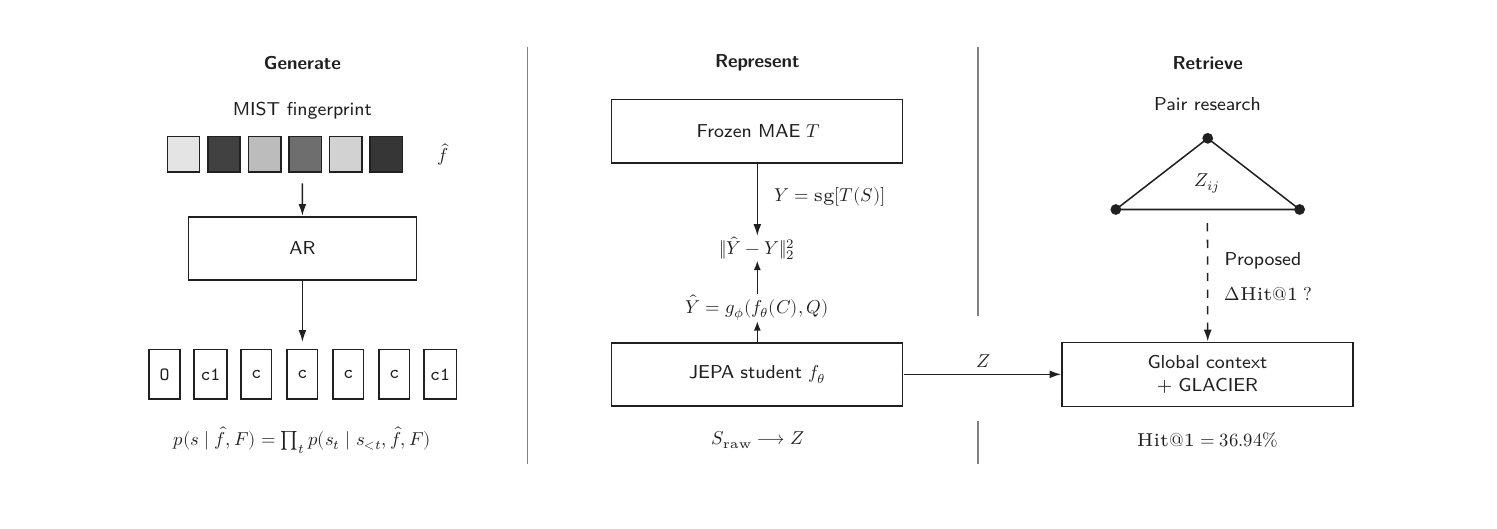
\begin{tikzpicture}[x=1cm,y=1cm,scale=1.14375,transform shape]
% Three column centres and a shared output baseline.
\coordinate (generate) at (3.05,6.46);
\coordinate (represent) at (8.10,6.46);
\coordinate (retrieve) at (13.10,6.46);
\foreach \name/\title in {generate/Generate,represent/Represent,retrieve/Retrieve}{
 \node[font=\brandmedium\figurefont,inner sep=0] at (\name) {\title};}
\draw[line,line width=.55pt] (5.55,6.64)--(5.55,2.00);
\draw[line,line width=.55pt] (10.55,6.64)--(10.55,3.65);
\draw[line,line width=.55pt] (10.55,2.48)--(10.55,2.00);

\node[small,inner sep=0] at (3.05,5.93) {MIST fingerprint};
\foreach \i/\shade in {0/12,1/85,2/30,3/65,4/20,5/90}{\draw[fill=ink!\shade,draw=ink,line width=.55pt] (1.55+\i*.45,5.25) rectangle +(.36,.39);}
\node[inner sep=0] at (4.60,5.44) {$\hat f$};
\node[box,text width=2.25cm,minimum height=.70cm,inner sep=4pt] (ar) at (3.05,4.40) {AR};
\draw[arr] (3.05,5.12)--(ar.north);
\coordinate (tokens) at (3.05,3.00);
\foreach \i/\t in {0/O,1/c1,2/c,3/c,4/c,5/c,6/c1}{\node[box,minimum width=.34cm,minimum height=.55cm,inner sep=2pt,small] at (1.52+\i*.51,3.00) {\texttt{\t}};}
\draw[arr] (ar.south)--($(tokens)+(0,.36)$);
\node[font=\figurefont,inner sep=0] at (3.05,2.27) {$p(s\mid\hat f,F)=\prod_t p(s_t\mid s_{<t},\hat f,F)$};

\node[box,text width=2.95cm,minimum height=.70cm,inner sep=4pt] (teacher) at (8.10,5.70) {Frozen MAE $T$};
\node[font=\figurefont,inner sep=0] (loss) at (8.10,4.40) {$\|\widehat Y-Y\|_2^2$};
\draw[arr] (teacher.south)--(loss.north);
\node[small,anchor=west,inner sep=0] at (8.28,4.97) {$Y=\operatorname{sg}[T(S)]$};
\node[small,inner sep=0] (prediction) at (8.10,3.74) {$\widehat Y=g_\phi(f_\theta(C),Q)$};
\node[box,text width=2.95cm,minimum height=.70cm,inner sep=4pt] (student) at (8.10,3.00) {JEPA student $f_\theta$};
\draw[-{Latex[length=1.2mm,width=.9mm]},line width=.55pt,draw=ink] (student.north)--(prediction.south);
\draw[-{Latex[length=1.2mm,width=.9mm]},line width=.55pt,draw=ink] (prediction.north)--(loss.south);
\node[inner sep=0] at (8.10,2.27) {$S_{\rm raw}\longrightarrow Z$};

\node[small,inner sep=0] at (13.10,6.00) {Pair research};
\coordinate (ra) at (12.08,4.83);
\coordinate (rb) at (14.12,4.83);
\coordinate (rc) at (13.10,5.62);
\draw[ink,line width=.55pt] (ra)--(rb)--(rc)--cycle;
\foreach \p in {ra,rb,rc}{\fill[ink] (\p) circle (.06);}
\node[small,inner sep=0] at (13.10,5.12) {$Z_{ij}$};
\node[box,text width=2.95cm,minimum height=.70cm,inner sep=4pt] (flare) at (13.10,3.00) {\small Global context\\+ GLACIER};
\draw[arr,dashed] (13.10,4.68)--(flare.north);
\node[small,anchor=west,inner sep=0] at (13.28,4.26) {Proposed};
\node[small,anchor=west,inner sep=0] at (13.28,3.89) {$\Delta\mathrm{Hit@1}\;?$};
\draw[arr] (student.east)--node[above,small] {$Z$}(flare.west);
\node[inner sep=0] at (13.10,2.27) {$\mathrm{Hit@1}=36.94\%$};
% Fixed canvas: 183 x 60.046875 mm. No clipping: overflow is audited.
\pgfresetboundingbox
\path[use as bounding box] (0,1.6) rectangle (16,6.85);
\end{tikzpicture}
\end{document}
